\documentclass{beamer}
\setbeamertemplate{footline}[page number]
\date{}
\author{}
\institute{}

%%%%%%% Put these names back in the final version 
%\\Aswathy Rajendra Kurup\\Meenu Ajith}
%\institute{Department of Electrical and Computer Engineering\\The University of New Mexico}
\setbeamercovered{transparent}
\usepackage{setspace}
\usepackage{array}
\usepackage[T1]{fontenc}
\usepackage{graphicx}
\usepackage{amsmath}
\usepackage{amsfonts}
\usepackage{amssymb}
\usepackage{makeidx}
\usefonttheme{serif}
\usepackage{multirow}
\usepackage{booktabs} 
\usepackage{rotating}
\usepackage{color}
\usepackage{float}
\usepackage[latin1]{inputenc}
\usepackage[english]{babel}
\usepackage{amsmath}
\usepackage{amsfonts}
\usepackage{eurosym}
\usepackage{rotating}
\usepackage{multicol}
\usepackage{pythonhighlight}
\usepackage[normalem]{ulem}
\newcommand{\ba}{{\bf a}}
\newcommand{\bb}{{\bf b}}
\newcommand{\bc}{{\bf c}}
\newcommand{\bd}{{\bf d}}
\newcommand{\be}{{\bf e}}
\newcommand{\bbf}{{\bf f}}
\newcommand{\bg}{{\bf g}}
\newcommand{\bh}{{\bf h}}
\newcommand{\bi}{{\bf i}}
\newcommand{\bk}{{\bf k}}
\newcommand{\bl}{{\bf l}}
\newcommand{\bm}{{\bf m}}
\newcommand{\bn}{{\bf n}}
\newcommand{\bo}{{\bf o}}
\newcommand{\bp}{{\bf p}}
\newcommand{\bq}{{\bf q}}
\newcommand{\br}{{\bf r}}
\newcommand{\bs}{{\bf s}}
\newcommand{\bt}{{\bf t}}
\newcommand{\bu}{{\bf u}}
\newcommand{\bv}{{\bf v}}
\newcommand{\bw}{{\bf w}}
\newcommand{\bx}{{\bf x}}
\newcommand{\by}{{\bf y}}
\newcommand{\bz}{{\bf z}}

\newcommand{\bA}{{\bf A}}
\newcommand{\bB}{{\bf B}}
\newcommand{\bC}{{\bf C}}
\newcommand{\bE}{{\bf E}}
\newcommand{\bG}{{\bf G}}
\newcommand{\bH}{{\bf H}}
\newcommand{\bI}{{\bf I}}
\newcommand{\bK}{{\bf K}}
\newcommand{\bL}{{\bf L}}
\newcommand{\bM}{{\bf M}}
\newcommand{\bO}{{\bf O}}
\newcommand{\bQ}{{\bf Q}}
\newcommand{\bR}{{\bf R}}
\newcommand{\bS}{{\bf S}}
\newcommand{\bT}{{\bf T}}
\newcommand{\bV}{{\bf V}}
\newcommand{\bW}{{\bf W}}
\newcommand{\bX}{{\bf X}}
\newcommand{\bY}{{\bf Y}}
\newcommand{\bZ}{{\bf Z}}
\newcommand\uptocnt{\stackrel{\mathclap{\normalfont\mbox{c}}}{\propto}}
\newcommand{\bpt}{{\bf pt}}
\newcommand{\bpl}{{\bf pl}}
\newcommand{\bdp}{{\bf dp}}
\newcommand{\btemp}{{\bf temp}}

\newcommand{\bmu}{{\boldsymbol \mu}}
\newcommand{\bSigma}{{\boldsymbol \Sigma}}
\newcommand{\bsigma}{{\boldsymbol \sigma}}
\newcommand{\bvarPhi}{{\boldsymbol \varPhi}}
\newcommand{\bvarphi}{{\boldsymbol \varphi}}
\newcommand{\bPhi}{{\boldsymbol \Phi}}
\newcommand{\bdelta}{{\boldsymbol \delta}}
\newcommand{\bZero}{{\bf 0}}
\newcommand{\bOne}{{\bf 1}}
\newcommand{\balpha}{{\boldsymbol \alpha}}
\newcommand{\bAlpha}{{\boldsymbol A}}
\newcommand{\btheta}{{\boldsymbol \theta}}

\newcommand{\softmax}{\text{softmax}}
\newcommand{\diag}{\text{diag}}
\newcommand{\sinc}{\mathrm{sinc}}
\newcommand{\argmin}{\mathop{\mathrm{argmin}}}
\newcommand{\infl}{\eta}
\newcommand{\Ind}{\mathrm{I}}
\newcommand{\Real}{\mathbb R}
\newcommand{\Intg}{\mathbb Z}
\newcommand{\Complex}{\mathbb C}
\newcommand{\Natural}{\mathbb N}
\newcommand{\Fourier}[1]{\mathcal{F} \{#1\}}
%\newcommand{\ii}{\mathbbm{i}}
\newcommand{\bphi}{\boldsymbol{\mathit{\phi}}}

\newcommand{\hs}{\hspace{2pt}}
\newcommand{\sign}{\text{sign}}
\author{Manel Mart\'inez-Ram\'on\\Meenu Ajith\\Aswathy Rajendra Kurup}

\usetheme{Madrid}
\usecolortheme{beaver}
\usepackage{tikz}
\usetikzlibrary{fit,arrows,calc,positioning}
\usepackage{listings}
\usepackage{xcolor}
\usepackage{emerald} 
\usepackage[T1]{fontenc} 
\usepackage{verbatim}
\usepackage{graphicx}
\usepackage{epsfig}
\usepackage{psfrag}
\usepackage[english]{babel}
\usepackage{listings}
\usepackage{courier}
\usepackage{color}
 \usepackage{vwcol} 
 \usepackage[english]{babel} % To obtain English text with the blindtext package
\usepackage{blindtext}
\definecolor{codegreen}{rgb}{0,0.6,0}
\definecolor{codegray}{rgb}{0.5,0.5,0.5}
\definecolor{codepurple}{rgb}{0.58,0,0.82}
\definecolor{backcolour}{rgb}{0.95,0.95,0.92}

\lstdefinestyle{mystyle}{
  backgroundcolor=\color{backcolour},   commentstyle=\color{codegreen},
  keywordstyle=\color{magenta},
  numberstyle=\tiny\color{codegray},
  stringstyle=\color{codepurple},
  basicstyle=\ttfamily\footnotesize,
  breakatwhitespace=false,         
  breaklines=true,                 
  captionpos=b,                    
  keepspaces=true,                 
  numbers=left,                    
  numbersep=5pt,                  
  showspaces=false,                
  showstringspaces=false,
  showtabs=false,                  
  tabsize=2
}
\lstset{style=mystyle}

%% Stuff for movies

% %\newcommand{\bt}{{\bf t}}
% \newcommand{\br}{{\bf r}}
% \newcommand{\bs}{{\bf s}}
% \newcommand{\by}{{\bf y}}
% \newcommand{\bz}{{\bf z}}
% \newcommand{\bx}{{\bf x}}
% \newcommand{\bw}{{\bf w}}
% \newcommand{\be}{{\bf e}}
% \newcommand{\bbf}{{\bf f}}
% \newcommand{\bb}{{\bf b}}
% \newcommand{\bd}{{\bf d}}
% \newcommand{\bA}{{\bf A}}
% \newcommand{\bB}{{\bf B}}
% \newcommand{\bL}{{\bf L}}
% \newcommand{\bM}{{\bf M}}

% \newcommand{\bC}{{\bf C}}
% \newcommand{\bI}{{\bf I}}
% \newcommand{\bK}{{\bf K}}
% \newcommand{\bk}{{\bf k}}
% \newcommand{\bT}{{\bf T}}
% \newcommand{\bV}{{\bf V}}
% \newcommand{\bW}{{\bf W}}
% \newcommand{\bX}{{\bf X}}
% \newcommand{\bY}{{\bf Y}}
% \newcommand{\bZ}{{\bf Z}}
% \newcommand{\bm}{{\bf m}}
% \newcommand{\bpt}{{\bf pt}}
% \newcommand{\bpl}{{\bf pl}}
% \newcommand{\bdp}{{\bf dp}}
% \newcommand{\btemp}{{\bf temp}}
% \newcommand{\bl}{{\bf l}}
% \newcommand{\bu}{{\bf u}}
% \newcommand{\bmu}{{\boldsymbol \mu}}
% \newcommand{\bSigma}{{\boldsymbol \Sigma}}
% \newcommand{\bLambda}{{\boldsymbol \Lambda}}

% \newcommand{\bsigma}{{\boldsymbol \sigma}}
% \newcommand{\bvarphi}{{\boldsymbol \varPhi}}
% \newcommand{\btheta}{{\boldsymbol \theta}}
% \newcommand{\bZero}{{\bf 0}}
% \newcommand{\balpha}{{\boldsymbol \alpha}}
% \newcommand{\bpi}{{\boldsymbol \pi}}
% \newcommand{\bxi}{{\boldsymbol \xi}}
% \newcommand{\bdelta}{{\boldsymbol \delta}}
\lstset{
	language=Python,
	basicstyle=\footnotesize\ttfamily\color{black},
	commentstyle = \footnotesize\ttfamily\color{red},
	keywordstyle=\footnotesize\ttfamily\color{blue},
	stringstyle=\footnotesize\ttfamily\color{black},
%	columns=fixed,
%	numbers=left,    
	numberstyle=\tiny,
	stepnumber=1,
	numbersep=5pt,
	tabsize=1,
	extendedchars=true,
	breaklines=true,            
	frame=b,         
	showspaces=false,
	showtabs=true,
	xleftmargin=6pt,
	framexleftmargin=6pt,
	framexrightmargin=2pt,
	framexbottommargin=4pt,
	showstringspaces=false      
}

\lstloadlanguages{
         Python
}

%\graphicspath{ {./images/} }  % Figures path - used in graphicx

%\selectcolormodel{cmyk}

\mode<presentation>

\newcommand{\dred}{darkred!90!black}
\newcommand{\written}{\ECFJD\textcolor{cyan!50!white}}
\newcommand{\hlight}{\textcolor{\dred}}
\newcommand{\Ex}{\textcolor{\dred}{Ex. }}

% remove navigation symbols in full screen mode
\setbeamertemplate{navigation symbols}{}  
\setbeamertemplate{blocks}[rounded][shadow=false]
\setbeamercolor{note page}{fg=black}

\setbeamercolor{title}{fg=\dred}
\setbeamercolor{frametitle}{fg=white}
\setbeamercolor{frametitle}{bg=\dred}
\setbeamercolor{structure}{fg=black,bg=white}
\setbeamercolor{background canvas}{bg=white,fg=black}
\setbeamercolor{normal text}{fg=black,bg=white}
\setbeamercolor{item}{fg=red!80!black,bg=white!}
\addtobeamertemplate{block begin}{\setbeamercolor{block title}{fg=white,bg=\dred}
\setbeamercolor{block body}{fg=white,bg=gray}}{}


\usepackage{algorithm,algorithmic}
\usepackage[algo2e]{algorithm2e} 
%\title{Lesson 1.1}
\title{2. Training practicalities}
\subtitle{}


\addtobeamertemplate{frametitle}{}


\begin{document}


\maketitle

\begin{frame}{Generalization and overfitting}
\begin{itemize}
    \item Purpose of training:  achieve the best possible test accuracy. 
    \item the training dataset must contain enough information about its structure.\item This is compromised as the number of samples decrease. 
    \item The difference between the training and test errors in a neural network with sufficient complexity is called \emph{overfitting}. 
    \item The ability to obtain a sufficiently low error both in training and test is called \emph{generalization} ability.   
\end{itemize}
\end{frame}

\begin{frame}{Example of overfitting}
    \begin{center}
    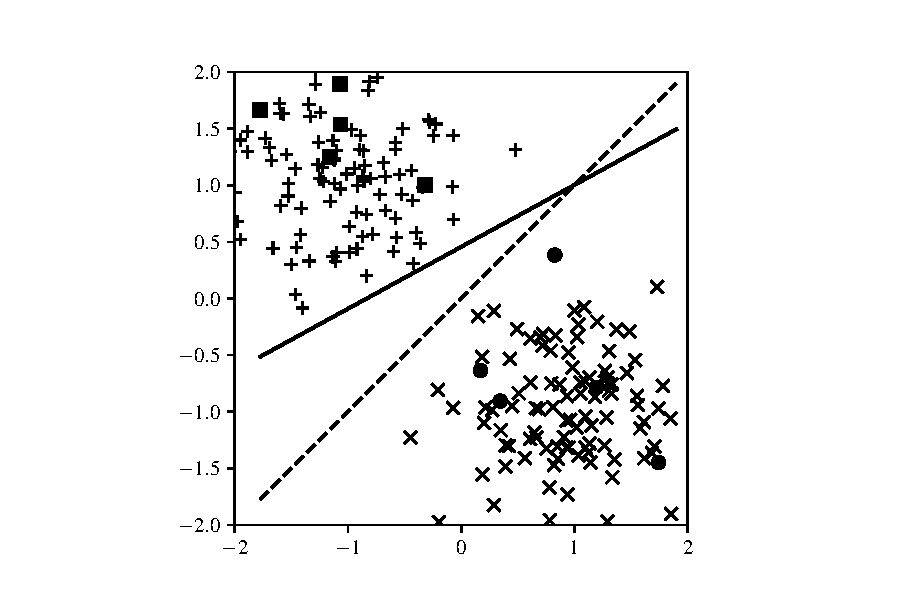
\includegraphics[scale=0.39]{Module 1 (NN)/pics/example_161_5_.pdf} 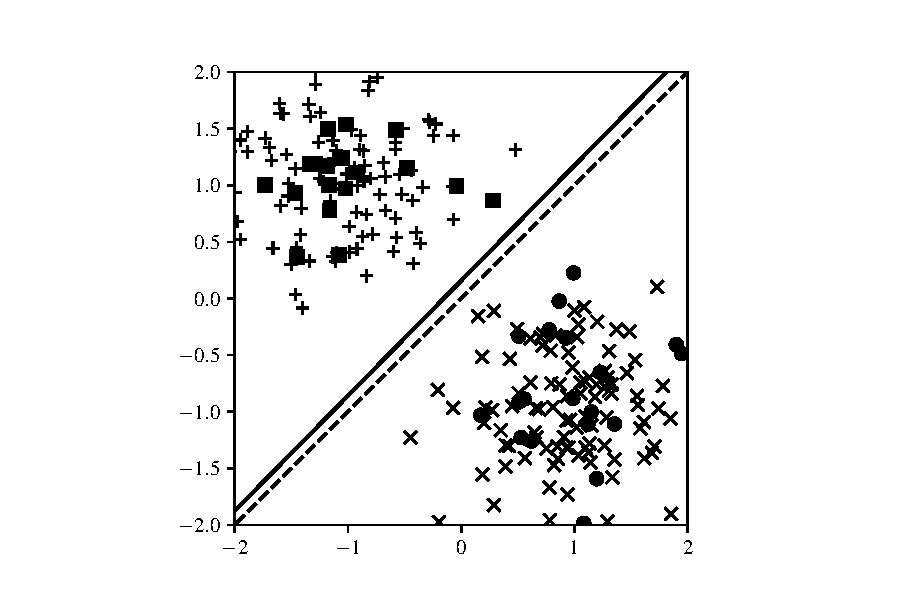
\includegraphics[scale=0.39]{Module 1 (NN)/pics/example_161_20_.pdf}
    \end{center}
\begin{itemize}
\item A classifier is trained with only the 10 samples highligthed as squares and dots (left). 
\item The resulting classifier is depicted as a solid line which is clearly biased with respect to the optimum.
\item As the number of training data increases, the classifier gets closer to the optimum (right).
\end{itemize}
\end{frame}

\begin{frame}{Learning curve}

\begin{center}
    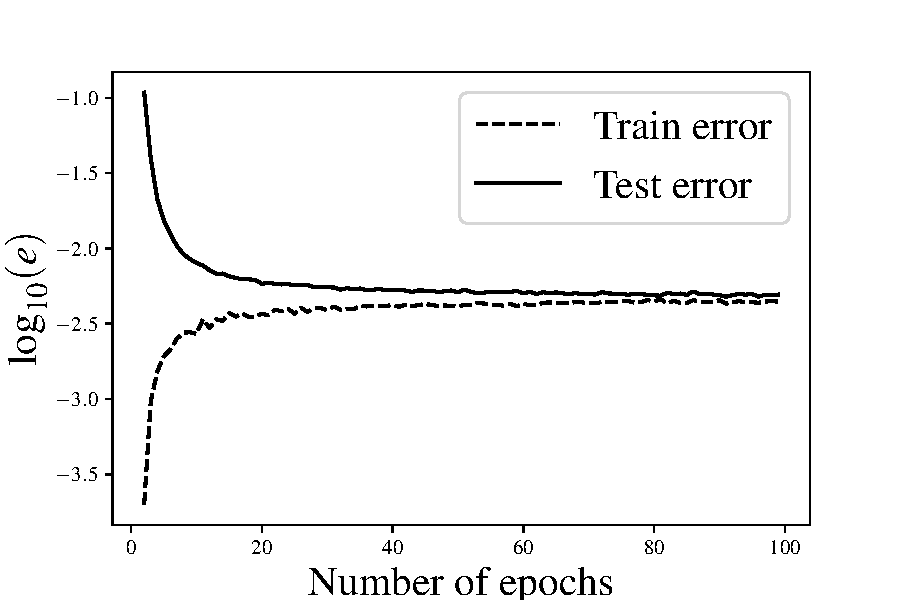
\includegraphics[scale=0.38]{Module 1 (NN)/pics/example_161_train_test_error100_.pdf}
    \end{center}
    
    Test error rate (continuous line) and train error rate (dashed line) as a function of the number of training samples for the previous  example.
\end{frame}

\begin{frame}{Parameter regularization}{Ridge regularization}
\begin{itemize}
    \item To reduce the overfitting we must increase the number of data. But this is impossible in almost all practical cases.
    \item The use of the $L_2$ or \emph{ridge regularization} is used to produce solutions with low parameter norm
    
    \begin{equation}\label{eq:reg_cross_entropy}
J(\boldsymbol \theta) = J_{ML}(\boldsymbol \theta) + \frac{\lambda}{2} \sum_{l} ||{\bf W}^{(l)}||_F^2
\end{equation}
where $\|\cdot \|^2_F$ is the Frobenius norm.
  
        \item Basic idea: emphasize the important nodes by decreasing the rest.
        \item This way we have \emph{simpler} solutions.
\item The gradient of the regularization is $\lambda \bW^{(l)}$, so at each iteration we decrease each parameter an equal \emph{fraction of its value}.
\end{itemize}
\end{frame}

\begin{frame}{Parameter regularization}{Lasso}
\begin{itemize}
    \item A different way to simplify the solution is to apply the $L_1$ or ``least absolute shrinkage and selection operator'' (lasso).
    
     \begin{equation}\label{eq:reg_cross_entropy}
J(\boldsymbol \theta) = J_{ML}(\boldsymbol \theta) + \lambda \sum_{l} ||{\bf W}^{(l)}||_1
\end{equation}
where $\|\cdot \|_1$ returns the absolute value of the elements of the matrix.  

\item The gradient of the regularization is simply $sign\left(\bW^{(l)}\right)$. At each iteration, all parameters are decreased an \emph{equal quantity} if they are not zero. 
\item This regularization sets some parameters to zero, and thus it \emph{selects} connections.
\end{itemize}
\end{frame}

\begin{frame}{Parameter regularization} {Elastic net}
\begin{itemize}
    \item Lasso regularization drops correlated variables, while ridge regression combines them to minimize the noise or uncertainty in their values. 
    \item An intermediate solution is to combine both
    
     \begin{equation}\label{eq:reg_cross_entropy}
J(\boldsymbol \theta) = J_{ML}(\boldsymbol \theta) + \lambda \left(  (1-\alpha)\sum_{l} ||{\bf W}^{(l)}||_F^2+ \alpha \sum_{l} ||{\bf W}^{(l)}||_1 \right)
\end{equation}
where $0 \leq \alpha \leq 1$.    
\end{itemize}
    
\end{frame}

\begin{frame}{Parameter regularization}{Comparisons}
\begin{center}
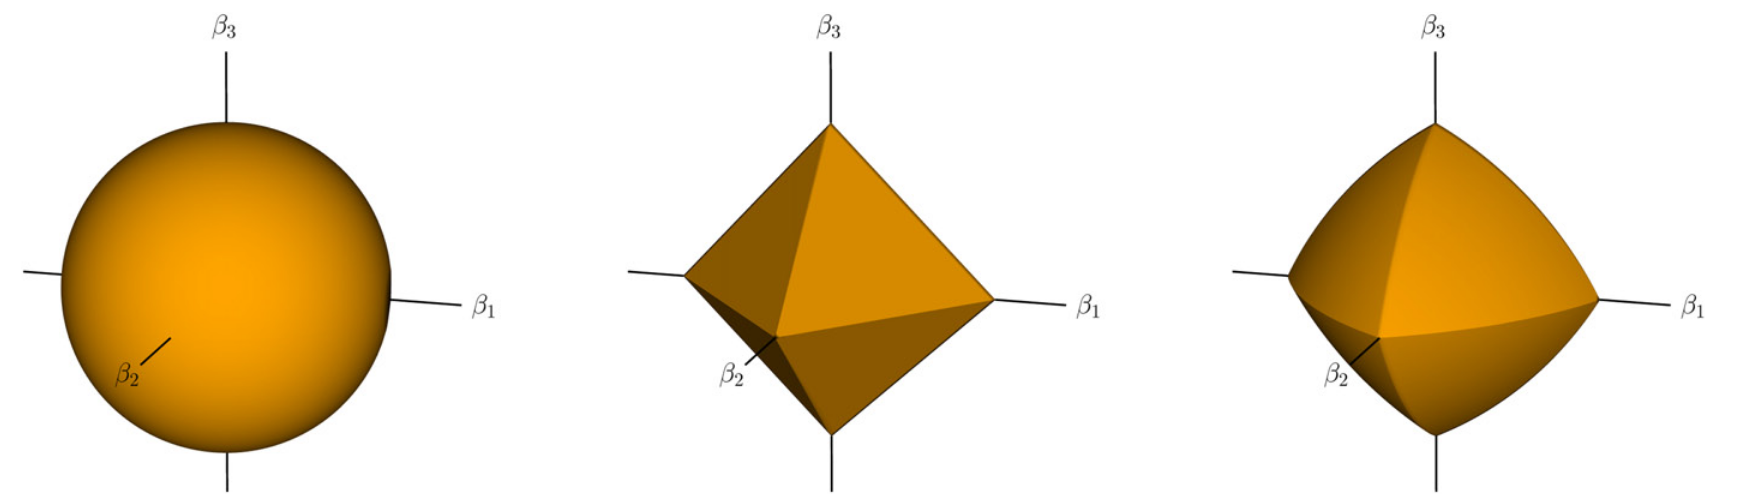
\includegraphics[scale=0.2]{Module 1 (NN)/pics/regularization_comparisons.png}
\end{center}
Constraint balls for ridge, lasso, and elastic-net. The sharp edges and corners of the latter two allow for  selection and shrinkage$^1$.

\vspace{1cm}

$^1$\footnotesize{Trevor Hastie, Technometrics 62.4 (2020), pp. 426-433.}. 
\end{frame}
\begin{frame}{Weight initializations}
\begin{itemize}

\item The convergence of a NN depends on a proper initialization.  

\item Xavier initialization:
\begin{itemize}
    \item   Xavier Glorot and Yoshua Bengio proposed$^1$ a Gaussian random initialization for sigmoidal activations with std  $\sigma =\frac{1}{\sqrt{D_{l-1}}}$
    \item Good results in neural networks with logistic and tanh activations.
    \item Many effects not understood. 
\end{itemize}  
\item He activation:
\begin{itemize}
\item He et al.$^2$ show that Xavier does not work well when hidden activations are ReLU. 
\item They proposed a standard deviation $\sigma =\sqrt{\frac{2}{{D_{l-1}}}}$. 
\end{itemize}
\end{itemize}
$^1$\footnotesize{Xavier Glorot and Yoshua Bengio. Proceeding sot the JMLR, 2010, pp. 249-256.}



$^2$\footnotesize{Kaiming He et al.  Proceedings of the IEEE ICCV, 2015, pp. 1026-1034.}

\end{frame}

\end{document}